% CVPR 2025-based 4+1 research-paper template.
\documentclass[10pt,twocolumn,letterpaper]{article}
\usepackage{cvpr}
%
% --- inline annotations
%
\newcommand{\red}[1]{{\color{red}#1}}
\newcommand{\todo}[1]{{\color{red}#1}}
\newcommand{\TODO}[1]{\textbf{\color{red}[TODO: #1]}}
% --- disable by uncommenting  
% \renewcommand{\TODO}[1]{}
% \renewcommand{\todo}[1]{#1}


\usepackage{amsmath,booktabs}


\definecolor{cvprblue}{rgb}{0.21,0.49,0.74}
\usepackage[pagebackref,breaklinks,colorlinks,allcolors=cvprblue]{hyperref}
\def\paperID{00000000}
\def\confName{Anonymous Review}
\def\confYear{2026}

\title{How Far Do Image-Level Labels Go for Localisation in Medical Anomaly Detection?}
\author{Anonymous authors\\Anonymous affiliation}

\begin{document}
\maketitle
\begin{abstract}
Pixel masks are costly, while image-level labels are common in medical anomaly detection. We test how far image-level supervision can support localization in MVFA under leave-one-modality-out evaluation on BMAD. A hybrid nnPU fine-tune does not show a consistent gain over matched fine-tuning: AUPRO is higher in 6 of 9 pairs (one-sided sign-test $p=0.2539$), with a target-specific Brain MRI signal. Fully mask-free nnPU retains a mean 0.583 of R0 pixel-AUROC margin; an unregistered top-$k$ MIL baseline retains 0.927--0.994 in single-seed observations. Lower-tail mixture-proportion estimates on masked-source patch scores range from $-0.286$ to $1.000$ against true fractions from 0.008 to 0.119. These results support an analysis of supervision limits, not a claim of improvement over MVFA.
\end{abstract}

\section{Introduction}
\label{sec:intro}
Vision-language models such as CLIP~\cite{clip2021} support zero-shot recognition, and MVFA adapts them to medical anomaly detection with multi-level visual adapters~\cite{huang2024mvfa}. Its localization training uses pixel masks, even though many benchmark sources provide only image labels~\cite{bmad2024}. This leaves a practical question: how much localization can image-level supervision provide when the target modality is unseen?

We study patch-level positive-unlabelled (PU) learning~\cite{elkan2008pu,kiryo2017nnpu} in MVFA under leave-one-modality-out evaluation on Brain MRI, Liver CT, and Retina RESC. Round 1 is an analysis of a controlled hybrid fine-tune, a fully mask-free PU model, and a top-$k$ multiple-instance-learning baseline. It does not support a general improvement claim.

Our contributions are:
\begin{itemize}
\item A matched comparison of hybrid nnPU fine-tuning and plain fine-tuning: no consistent AUPRO gain across targets, with a Brain-specific signal.
\item A prior-estimation failure analysis against known masked-source patch fractions, showing that the score distributions violate the mixture-proportion assumptions used by MPE~\cite{ramaswamy2016mpe}.
\item An unregistered mask-free top-$k$ MIL observation that retains much of R0 pixel AUROC; single-seed results outside Liver limit this evidence.
\end{itemize}

Task 3's audit also found that the released zero-shot pipeline uses source test folders and selects R0 checkpoints using target-test performance; we report this inherited selection bias explicitly.

\section{Related Work}
\label{sec:related}
\subsection{Medical anomaly detection and vision-language adaptation}
Medical anomaly benchmarks span diverse modalities and label regimes~\cite{medicalad_survey2021,bmad2024}. CLIP-based methods including WinCLIP, APRIL-GAN, AnomalyCLIP, AdaCLIP, and VCP-CLIP adapt visual-language representations for anomaly detection~\cite{winclip2023,aprilgan2023,anomalyclip2023,adaclip2024,vcpclip2024}. Medical variants such as MediCLIP, IQE-CLIP, and MADPOT target clinical images~\cite{mediclip2024,iqeclip2026,madpot2026}. MVFA uses multi-level adapters and pixel-wise alignment for cross-modality medical anomaly detection~\cite{huang2024mvfa}. We study its dependence on masks during localization training.

\subsection{Weakly supervised and mask-free anomaly localisation}
Image-level supervision has been explored through cycle-consistent segmentation, attention-based MIL, and top-$k$ feature adaptation~\cite{cycle_seg2021,ilse2018attentionmil,adfa2023}; recent work also studies reasoning-driven localization~\cite{imagelevel2026}. Industrial anomaly detection provides common datasets and metrics~\cite{mvtec2019}. These methods use different protocols, so we do not compare their reported scores numerically.

\subsection{Positive-unlabelled learning and mixture-proportion estimation}
PU learning estimates a classifier from labeled positives and unlabeled mixtures~\cite{elkan2008pu}; nnPU constrains the estimated negative risk to be non-negative~\cite{kiryo2017nnpu}. Mixture-proportion estimation recovers the positive fraction only under irreducibility conditions~\cite{ramaswamy2016mpe}. We test those conditions on MVFA patch scores against known source mask fractions.

\section{Problem Formulation}
\label{sec:problem}
Let each source image contain $K$ patches with differential anomaly logits $z_k=s_1(x_k)-s_0(x_k)$. Normal-image patches follow $p_0$; patches from abnormal images are unlabeled and follow
\begin{equation}
p_U=\pi p_1+(1-\pi)p_0,
\label{eq:mixture_dist}
\end{equation}
where $p_1$ is the anomalous-patch distribution and $\pi$ is its fraction in $U$. Estimating $\pi$ from distributions requires irreducibility: $p_1$ cannot contain $p_0$ as a proper sub-mixture. The assumption is tested empirically below.

For binary loss $\ell(z,y)$, the non-negative PU risk is
\begin{equation}
R_{\rm nnPU}=(1-\pi)\mathbb{E}_N\ell(z,0)+\max\{0,\mathbb{E}_U\ell(z,1)-(1-\pi)\mathbb{E}_N\ell(z,1)\}.
\label{eq:nnpu_risk}
\end{equation}
The hybrid objective adds $\lambda R_{\rm nnPU}$ on mask-less sources to MVFA's Dice+Focal mask loss on masked sources; its control omits the PU term. Fully mask-free $M$ uses nnPU with fixed $\pi$, while $B0$ uses top-$k$ MIL with $k=\max(3,0.01K)$. Retention is the pixel-AUROC margin above chance divided by the R0 margin; chance is 50 points on the percent scale.

\section{Methodology}
\label{sec:method}
\subsection{Dataset}
BMAD contains six datasets; three have masks and three provide only image labels~\cite{bmad2024}. Leave-one-modality-out targets are Brain MRI, Liver CT, and Retina RESC. Each source is capped at 500 normal and 500 abnormal training images; the frozen backbone is CLIP ViT-L/14 with four adapter levels. A held-out 10\% source split is used for prior estimation. We report image AUROC, pixel AUROC, and AUPRO at FPR $0.30$.

\subsection{Approach}
M-h warm-starts segmentation adapters from R0 and trains for 2,000 steps with MVFA mask loss on masked sources plus $\lambda R_{\rm nnPU}$ on mask-less sources. Its $\pi$ is the mean true patch fraction from masked-source masks (D1); M-h-ctrl follows the same schedule without PU. Fully mask-free $M$ and $B0$ reinitialize both adapter sets; $M$ uses fixed $\pi=0.30$, and $B0$ uses top-$k$ MIL. Fine-tunes use the last checkpoint without target-test selection. The released R0 checkpoint was selected on target-test performance.

\begin{figure}[t]
  \centering
  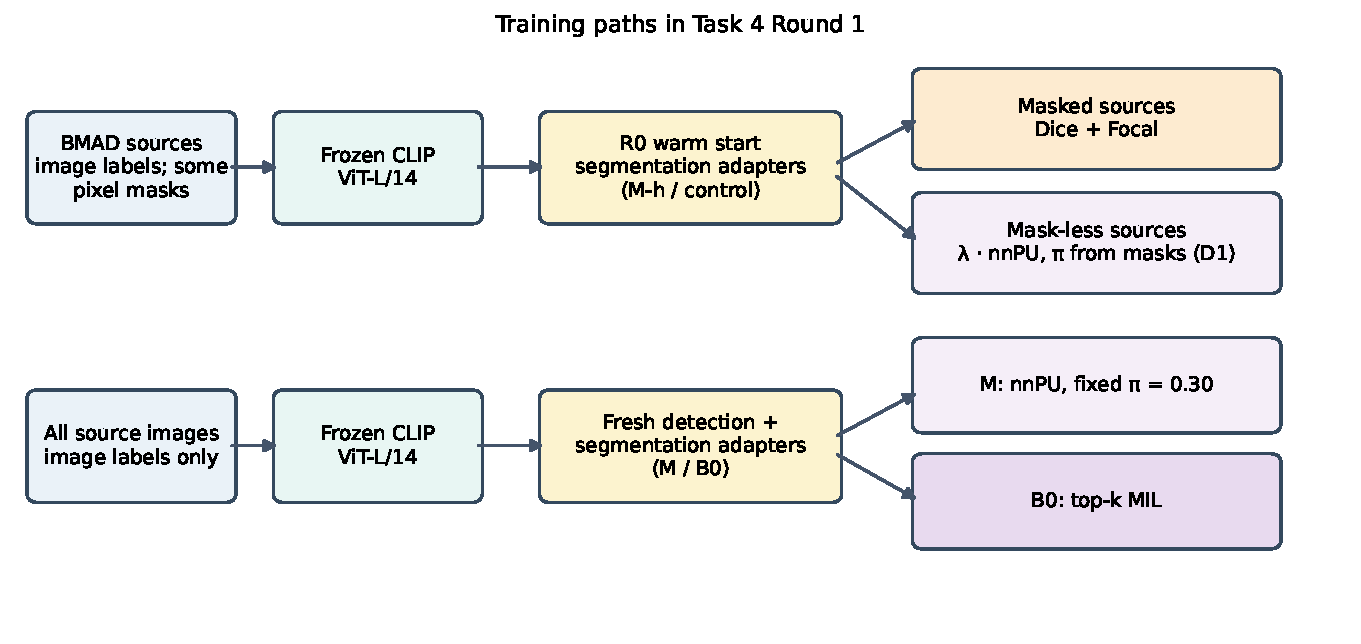
\includegraphics[width=\linewidth]{figures/fig1_method.pdf}
  \caption{Round 1 training paths. M-h combines the masked-source loss with nnPU on mask-less sources; M and B0 retrain both adapter sets without masks.}
  \label{fig:method}
\end{figure}

\section{Experiments}
\label{sec:experiments}
\subsection{Setup and hybrid comparison}
All runs are zero-shot leave-one-modality-out; M-h and its control use three matched seeds. Table~\ref{tab:hybrid_results} shows that M-h has higher AUPRO in 6 of 9 pairs (one-sided sign-test $p=0.2539$), below the registered criterion. The mean paired differences are $+5.20$ on Brain, $+0.33$ on Liver, and $+0.51$ on RESC; Brain is positive in all three seeds. M-h exceeds R0 only on Brain. R0's released checkpoint selection used target-test performance, whereas our fine-tunes did not.

\begin{table*}[t]
\centering
\small
\begin{tabular}{@{}llccc@{}}
\toprule
\textbf{Target Modality} & \textbf{Model} & \textbf{Image AUROC (\%)} & \textbf{Pixel AUROC (\%)} & \textbf{AUPRO (\%)} \\
\midrule
Liver CT & R0 (published) & 76.24 & 97.85 & — \\
Liver CT & R0 (reproduced) & 81.19 & 97.92 & 92.34 \\
Liver CT & $M\text{-}h$ (PU fine-tune) & $80.29 \pm 0.63$ & $96.97 \pm 0.18$ & $91.39 \pm 0.27$ \\
Liver CT & $M\text{-}h\text{-ctrl}$ (matched control) & $81.63 \pm 0.37$ & $96.99 \pm 0.31$ & $91.07 \pm 0.41$ \\
\midrule
Brain MRI & R0 (published) & 78.63 & 90.27 & — \\
Brain MRI & R0 (reproduced) & 79.80 & 89.68 & 65.35 \\
Brain MRI & $M\text{-}h$ (PU fine-tune) & $80.25 \pm 0.72$ & $91.71 \pm 0.71$ & $71.57 \pm 2.07$ \\
Brain MRI & $M\text{-}h\text{-ctrl}$ (matched control) & $80.31 \pm 0.96$ & $90.05 \pm 0.74$ & $66.38 \pm 2.12$ \\
\midrule
Retina RESC & R0 (published) & 83.31 & 92.05 & — \\
Retina RESC & R0 (reproduced) & 88.99 & 90.44 & 68.75 \\
Retina RESC & $M\text{-}h$ (PU fine-tune) & $89.20 \pm 0.16$ & $88.76 \pm 2.69$ & $67.45 \pm 6.15$ \\
Retina RESC & $M\text{-}h\text{-ctrl}$ (matched control) & $88.92 \pm 0.08$ & $89.76 \pm 0.46$ & $66.94 \pm 1.14$ \\
\bottomrule
\end{tabular}
\caption{Hybrid fine-tuning versus the matched control. R0 is shown as published and reproduced; M-h and M-h-ctrl report mean $\pm$ sample SD over 3 seeds.}
\label{tab:hybrid_results}
\end{table*}
\subsection{Mask-free models and prior failure}
Table~\ref{tab:maskfree_results} shows that mask-free nnPU $M$ has mean seed-0 pixel-retention 0.583 across targets. Its Liver pixel AUROC is $59.45\pm15.51$; the high variance and fixed $\pi=0.30$ limit interpretation. The unregistered $B0$ baseline retains 0.927--0.994 of R0 pixel AUROC; results outside Liver are single-seed. Figure~\ref{fig:heatmaps} shows the fixed Liver examples.

\begin{table*}[t]
\centering
\small
\begin{tabular}{@{}llcc@{}}
\toprule
\textbf{Target} & \textbf{Model} & \textbf{Pixel AUROC (retention)} & \textbf{AUPRO (ratio)} \\
\midrule
Liver & $M$ (nnPU) & $59.45\pm15.51$ ($-0.002$) & $26.28\pm15.50$ (0.188) \\
Liver & $B0$ (top-$k$ MIL) & 94.42 (0.927) & 85.47 (0.926) \\
Brain & $M$ (nnPU) & 89.87 (1.005) & 64.50 (0.987) \\
Brain & $B0$ (top-$k$ MIL) & 89.46 (0.994) & 64.53 (0.987) \\
RESC & $M$ (nnPU) & 80.13 (0.745) & 58.52 (0.851) \\
RESC & $B0$ (top-$k$ MIL) & 89.57 (0.978) & 67.29 (0.979) \\
\bottomrule
\end{tabular}
\caption{Fully mask-free localization. Parentheses give pixel-AUROC retention and AUPRO/R0 ratio. Liver M is mean $\pm$ sample SD over 3 seeds; all other rows are single-seed.}
\label{tab:maskfree_results}
\end{table*}

\begin{figure}[t]
  \centering
  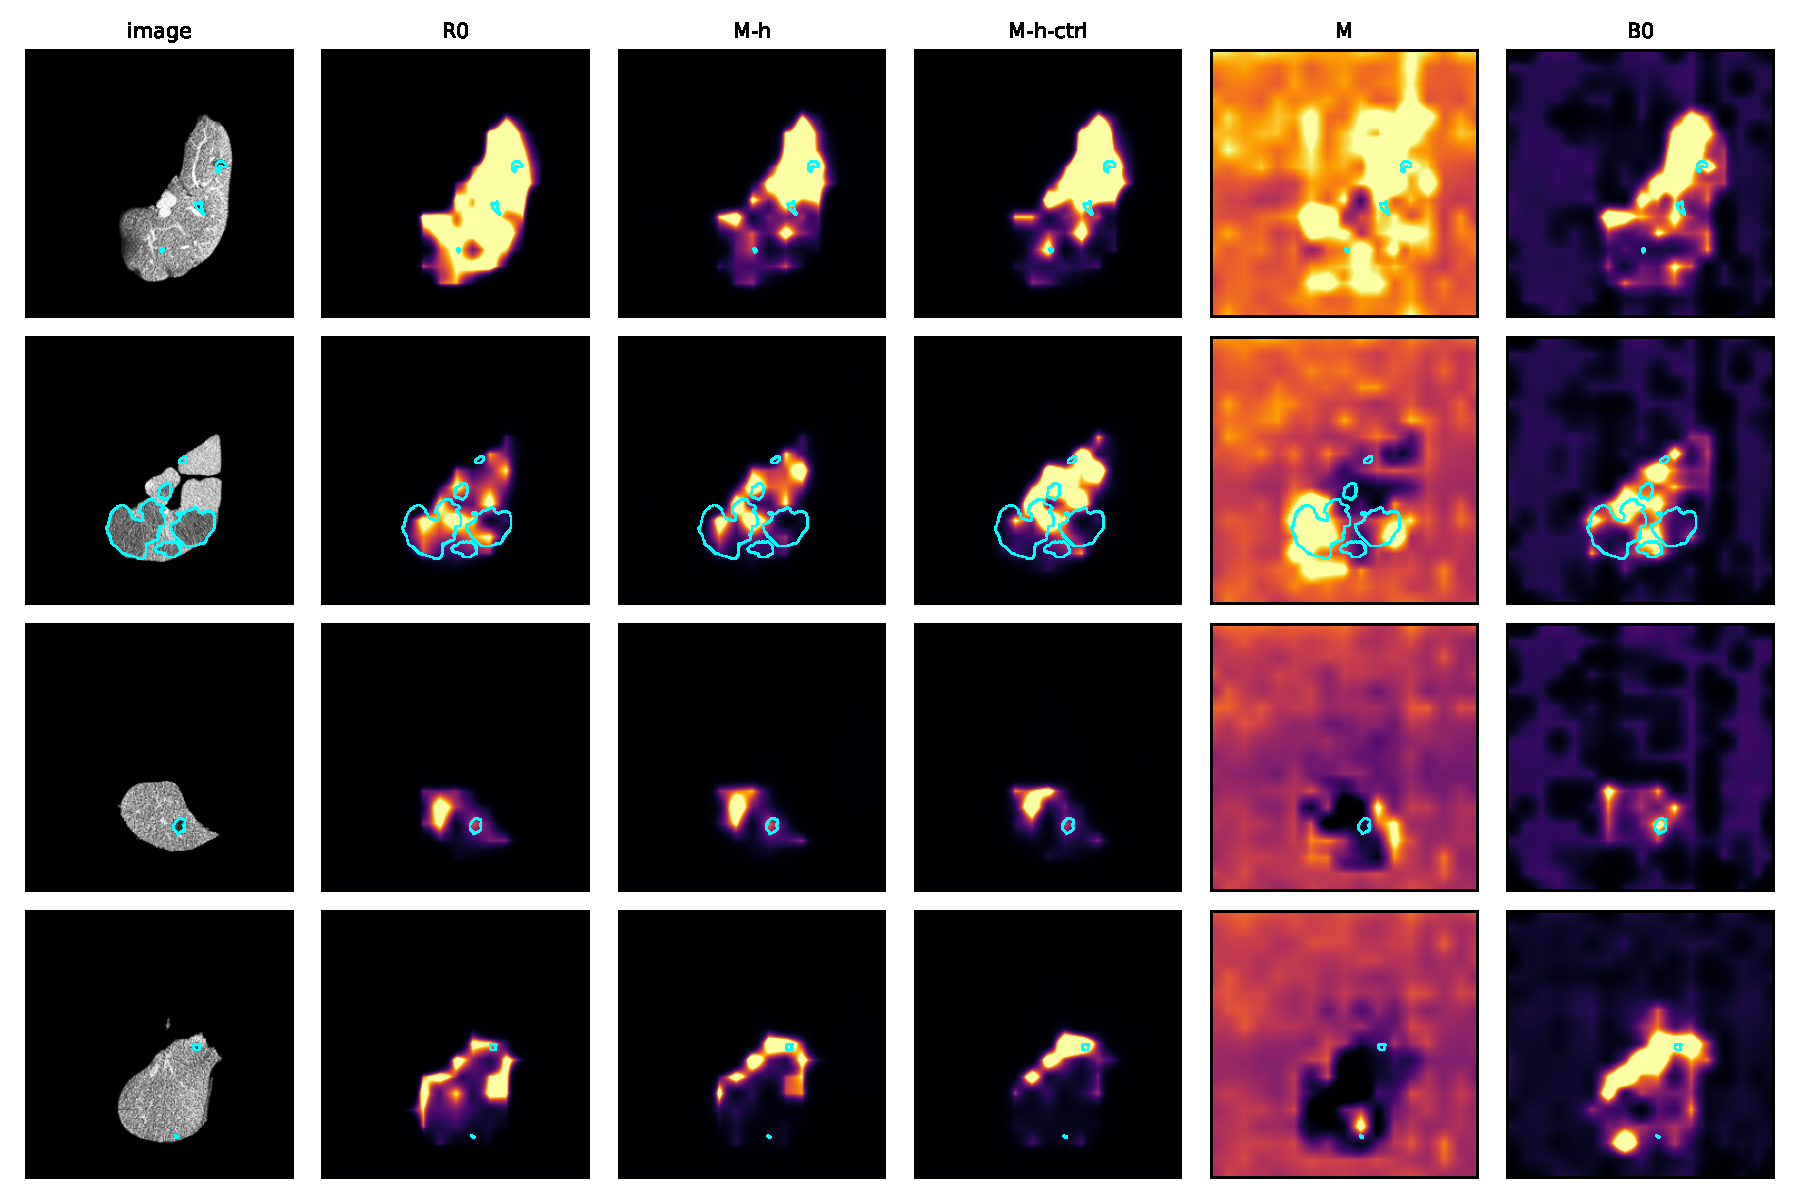
\includegraphics[width=\linewidth]{figures/fig2_liver_heatmaps.pdf}
  \caption{The same preselected Liver CT images and heat-map scale are shown for R0, M-h, M-h-ctrl, M, and B0.}
  \label{fig:heatmaps}
\end{figure}
True masked-source patch fractions range from 0.008 to 0.119, while raw lower-tail MPE estimates at the deepest level range from $-0.286$ to $1.000$. This failure indicates that the score distributions do not satisfy the estimator's irreducibility assumption. A Liver $M$ run with $\pi=0.05$ reached pixel AUROC 97.14 and AUPRO 87.28, but this override was selected after inspecting mask statistics and is post hoc.

\clearpage
\subsection{Interpretation}
The results distinguish the hybrid and fully mask-free settings. M-h retains the released segmentation-adapter warm start and uses masks through D1; it therefore tests whether PU loss on mask-less sources adds value alongside existing mask supervision. Its target-level pattern is not uniform: the Brain AUPRO difference is positive across seeds, while the Liver and RESC means are small and the cross-target sign test is inconclusive. The registered analysis framing is consequently the appropriate one.

The from-scratch models answer a separate question. M's mean retention of 0.583 is pulled down by unstable Liver results, whereas the single-seed B0 rows lie close to R0 in pixel-AUROC retention. This supports testing simple MIL further, but one seed on two targets cannot establish its expected performance. The sensitivity run with $\pi=0.05$ is not a fair substitute for the fixed-$\pi$ result because the value was chosen after inspecting mask statistics.

The prior-estimation result is similarly scoped: it shows failure on MVFA's observed patch-score distributions and masked-source labels, not a general impossibility of MPE. For this implementation, the estimates at the deepest level span negative values and 1.000 despite known fractions in the interval reported above. The evidence motivates calibrated score models or alternative priors as future work; neither is evaluated here.

\subsection{Limitations and scope}
The two supervision regimes answer different questions: M-h uses the mean true patch fraction from masked-source masks (D1), whereas fully mask-free M uses fixed $\pi=0.30$ (D2). Their comparison therefore does not isolate a mask-free effect. The experiment is also limited to a subsampled source pool and three held-out targets. M and B0 have only one seed outside Liver, so their near-R0 pixel retention is an observation, not a reliable estimate of expected performance. RESC shares the retinal OCT modality with OCT2017 in the source pool, limiting its interpretation as a fully unseen modality. Liver pixel AUROC is dominated by the normal background, and the high variance of M further weakens that metric. Finally, R0 inherits target-test checkpoint selection bias, while our fine-tunes use their last checkpoint. The Task 3 audit also found mask gradients reaching detection adapters in the released code. Together these factors constrain the strength and scope of conclusions.

\section{Conclusion}
\label{sec:conclusion}
On Round 1, hybrid nnPU fine-tuning does not yield a consistent localization gain, and data-driven prior estimation fails on MVFA patch scores. Top-$k$ MIL is a promising but unregistered observation that requires multi-seed confirmation. These results characterize the limits of image-level supervision under this protocol and do not establish improvement over MVFA.

\noindent\textbf{AI-use disclosure.} Tasks 1--4 used AI-augmented literature review, limitation extraction, ideation, and codification; PaperOrchestra drafted this manuscript, followed by artifact-based verification and manual revision.

\clearpage
{\small
\bibliographystyle{ieeenat_fullname}
\bibliography{references}
}
\end{document}